\documentclass{article}
\usepackage[paperwidth=370pt,paperheight=270pt,margin=0pt,noheadfoot]{geometry}
\usepackage{tikz}
\usetikzlibrary{calc}

\definecolor{ink}{RGB}{28,41,56}
\definecolor{axis}{RGB}{100,116,139}
\definecolor{grid}{RGB}{203,213,225}
\definecolor{curve}{RGB}{30,64,175}
\definecolor{teal}{RGB}{13,148,136}
\definecolor{tealfill}{RGB}{176,227,219}
% Integral diagrams have one consistent three-colour vocabulary: blue for an
% under-only part, yellow for an over-only (or still-unresolved) part, and
% green for their common part.  The common part is explicit rather than an
% alpha blend, so it remains visibly distinct after GIF palette quantization.
\definecolor{cyan}{RGB}{0,84,134}
\definecolor{cyanfill}{RGB}{0,114,178}
\definecolor{yellow}{RGB}{184,134,11}
\definecolor{yellowfill}{RGB}{240,228,66}
\definecolor{overlap}{RGB}{15,110,67}
\definecolor{overlapfill}{RGB}{20,153,92}
\definecolor{orange}{RGB}{234,88,12}
\definecolor{orangefill}{RGB}{254,215,170}
\definecolor{purple}{RGB}{126,34,206}
\definecolor{yellowedge}{RGB}{202,138,4}
\definecolor{projection}{RGB}{148,163,184}
\colorlet{under}{cyan}
\colorlet{underfill}{cyanfill}
\colorlet{over}{yellow}
\colorlet{overfill}{yellowfill}
\colorlet{shared}{overlap}
\colorlet{sharedfill}{overlapfill}
\colorlet{gap}{yellow}
\colorlet{gapfill}{yellowfill}

\pagestyle{empty}
\setlength\parindent{0pt}
\setlength\topskip{0pt}
\begin{document}
\noindent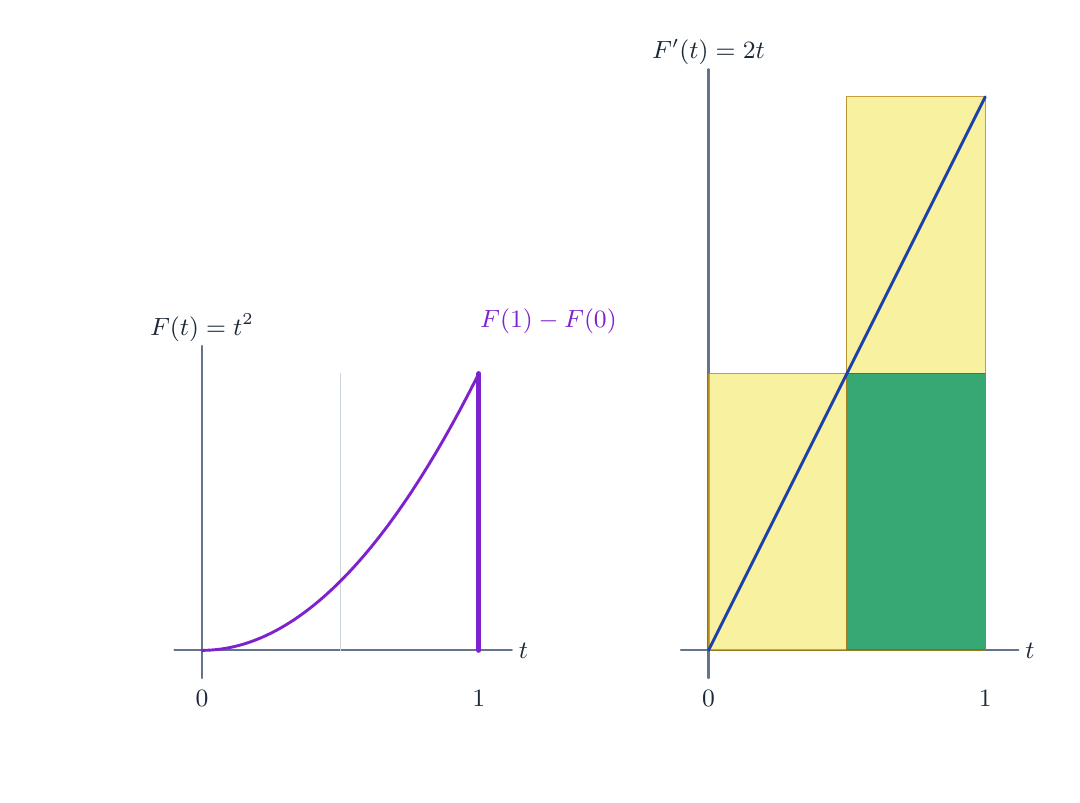
\begin{tikzpicture}[baseline=(current bounding box.north),x=1pt,y=1pt,line cap=round,line join=round]
\useasboundingbox (0,0) rectangle (370,270);
\draw[axis,line width=.75pt] (53,45) -- (175,45);
\draw[axis,line width=.75pt] (63,35) -- (63,155);
\draw[grid,line width=.3pt] (113.0,45) -- (113.0,145);
\node[font=\small,text=ink,anchor=north] at (63,34) {$0$};
\node[font=\small,text=ink,anchor=north] at (163,34) {$1$};
\node[font=\small,text=ink,anchor=south] at (63,153) {$F(t)=t^2$};
\draw[axis,line width=.75pt] (236,45) -- (358,45);
\draw[axis,line width=.75pt] (246,35) -- (246,255);
\draw[grid,line width=.3pt] (296.0,45) -- (296.0,245);
\node[font=\small,text=ink,anchor=north] at (246,34) {$0$};
\node[font=\small,text=ink,anchor=north] at (346,34) {$1$};
\node[font=\small,text=ink,anchor=south] at (246,253) {$F'(t)=2t$};
\draw[purple,line width=1.05pt] plot[smooth] coordinates {(63,45) (64,45.01) (65,45.04) (66,45.09) (67,45.16) (68,45.25) (69,45.36) (70,45.49) (71,45.64) (72,45.81) (73,46) (74,46.21) (75,46.44) (76,46.69) (77,46.96) (78,47.25) (79,47.56) (80,47.89) (81,48.24) (82,48.61) (83,49) (84,49.41) (85,49.84) (86,50.29) (87,50.76) (88,51.25) (89,51.76) (90,52.29) (91,52.84) (92,53.41) (93,54) (94,54.61) (95,55.24) (96,55.89) (97,56.56) (98,57.25) (99,57.96) (100,58.69) (101,59.44) (102,60.21) (103,61) (104,61.81) (105,62.64) (106,63.49) (107,64.36) (108,65.25) (109,66.16) (110,67.09) (111,68.04) (112,69.01) (113,70) (114,71.01) (115,72.04) (116,73.09) (117,74.16) (118,75.25) (119,76.36) (120,77.49) (121,78.64) (122,79.81) (123,81) (124,82.21) (125,83.44) (126,84.69) (127,85.96) (128,87.25) (129,88.56) (130,89.89) (131,91.24) (132,92.61) (133,94) (134,95.41) (135,96.84) (136,98.29) (137,99.76) (138,101.25) (139,102.76) (140,104.29) (141,105.84) (142,107.41) (143,109) (144,110.61) (145,112.24) (146,113.89) (147,115.56) (148,117.25) (149,118.96) (150,120.69) (151,122.44) (152,124.21) (153,126) (154,127.81) (155,129.64) (156,131.49) (157,133.36) (158,135.25) (159,137.16) (160,139.09) (161,141.04) (162,143.01) (163,145)};
\draw[purple,line width=1.8pt] (163,45) -- (163,145);
\path[fill=sharedfill,fill opacity=.85] (246,45) rectangle (296,45);
\path[fill=overfill,fill opacity=.5] (246,45) rectangle (296,145);
\draw[under,draw opacity=.8,line width=0.4pt] (246,45) rectangle (296,45);
\draw[over,draw opacity=.8,line width=0.4pt] (246,45) rectangle (296,145);
\path[fill=sharedfill,fill opacity=.85] (296,45) rectangle (346,145);
\path[fill=overfill,fill opacity=.5] (296,145) rectangle (346,245);
\draw[under,draw opacity=.8,line width=0.4pt] (296,45) rectangle (346,145);
\draw[over,draw opacity=.8,line width=0.4pt] (296,45) rectangle (346,245);
\draw[curve,line width=1.05pt] plot coordinates {(246,45) (247,47) (248,49) (249,51) (250,53) (251,55) (252,57) (253,59) (254,61) (255,63) (256,65) (257,67) (258,69) (259,71) (260,73) (261,75) (262,77) (263,79) (264,81) (265,83) (266,85) (267,87) (268,89) (269,91) (270,93) (271,95) (272,97) (273,99) (274,101) (275,103) (276,105) (277,107) (278,109) (279,111) (280,113) (281,115) (282,117) (283,119) (284,121) (285,123) (286,125) (287,127) (288,129) (289,131) (290,133) (291,135) (292,137) (293,139) (294,141) (295,143) (296,145) (297,147) (298,149) (299,151) (300,153) (301,155) (302,157) (303,159) (304,161) (305,163) (306,165) (307,167) (308,169) (309,171) (310,173) (311,175) (312,177) (313,179) (314,181) (315,183) (316,185) (317,187) (318,189) (319,191) (320,193) (321,195) (322,197) (323,199) (324,201) (325,203) (326,205) (327,207) (328,209) (329,211) (330,213) (331,215) (332,217) (333,219) (334,221) (335,223) (336,225) (337,227) (338,229) (339,231) (340,233) (341,235) (342,237) (343,239) (344,241) (345,243) (346,245)};
\node[font=\small,text=ink,anchor=south west,text=purple] at (160,156) {$F(1)-F(0)$};
\node[font=\small,text=ink,anchor=west] at (174,45) {$t$};
\node[font=\small,text=ink,anchor=west] at (357,45) {$t$};
\end{tikzpicture}
\end{document}
